\section{Introducción a los Sistemas de Archivos Distribuidos}

Los Sistemas de Archivos Distribuidos (DFS) son fundamentales para manejar grandes volúmenes de datos en múltiples ubicaciones. Estos sistemas permiten el acceso y la gestión de archivos almacenados en una red de nodos interconectados, lo cual es esencial para aplicaciones que requieren un gran ancho de banda y capacidad de almacenamiento, como el procesamiento de big data y la analítica de datos a gran escala.

\section{Historia y Evolución}

El concepto de DFS surge como una necesidad para manejar cantidades crecientes de datos y para proporcionar un acceso más rápido y confiable a estos datos, superando las limitaciones de los sistemas de archivos locales. Entre los primeros sistemas DFS se incluyen NFS (Network File System) y AFS (Andrew File System). Estos sistemas allanaron el camino para desarrollos más avanzados como GFS y HDFS, diseñados para satisfacer las demandas de aplicaciones de procesamiento de datos a gran escala.

\section{Google File System (GFS)}

\begin{figure}[H]
    \centering
    \begin{subfigure}[b]{0.5\textwidth}
        \centering
        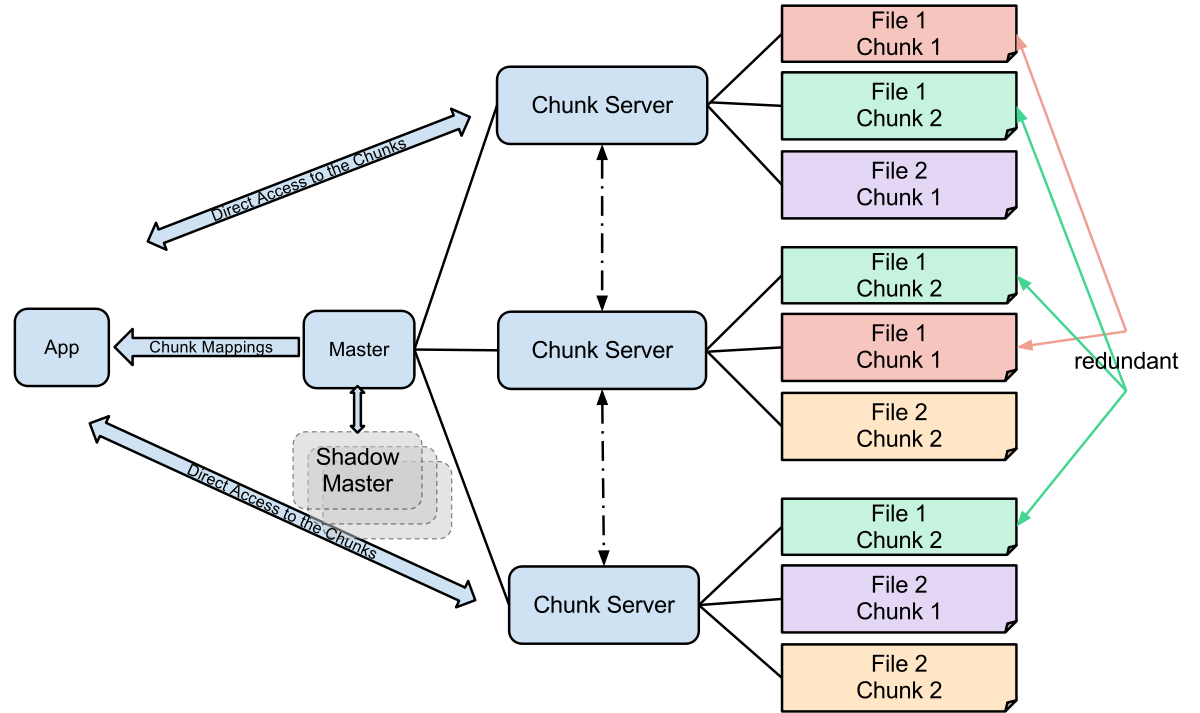
\includegraphics[width=\textwidth]{Figures/1. Content/GoogleFileSystemGFS.png}
        \caption{Google File System (GFS) Overview Architecture}
        \label{fig: GFSArchitecture}
    \end{subfigure}
    \hfill
\end{figure}

El Google File System (GFS) es un DFS diseñado para sistemas de alta escala utilizados por Google. GFS se caracteriza por su alta tolerancia a fallos y su eficacia en el manejo de grandes cantidades de datos, lo que lo hace ideal para aplicaciones que requieren el procesamiento de una gran cantidad de información de manera rápida y confiable. GFS también utiliza un enfoque innovador en la coherencia y replicación de datos para asegurar la disponibilidad y la integridad de los datos.

\subsection{Principios Clave de GFS}

El Google File System (GFS) se distingue por su diseño adaptado a aplicaciones que manejan grandes cantidades de datos. La arquitectura de GFS se basa en tres componentes principales: un único servidor maestro (Master), múltiples servidores chunk (Chunkservers), y los clientes que acceden al sistema.

\subsubsection{Arquitectura:}

\begin{itemize}
    \item \textbf{Master Server:} Gestiona el espacio de nombres del sistema de archivos, controla el mapeo de los archivos a chunks (bloques de datos), y administra las operaciones de control sobre los chunks. Mantiene toda la metadata en RAM para un acceso rápido.
    \item \textbf{ChunkServers}: Almacenan los chunks (normalmente de 64 MB) en discos locales y sirven las solicitudes de lectura y escritura de los clientes. Los chunks se replican en varios ChunkServers para garantizar la tolerancia a fallos.
\end{itemize}

\subsubsection{Coherencia y Replicación:}

\begin{itemize}
    \item GFS utiliza un modelo de coherencia relajado, donde las modificaciones concurrentes podrían resultar en versiones temporales no consistentes de los datos. Sin embargo, mediante la generación de versiones y la propagación de actualizaciones, GFS asegura la consistencia final de los datos.
    \item La replicación de chunks en múltiples ChunkServers mejora la disponibilidad y la fiabilidad. GFS también implementa un mecanismo de recuperación rápida en caso de fallos de nodos.
\end{itemize}

\subsubsection{Características útiles para el desarrollo de "Azeroth Nodes":}

\begin{itemize}
    \item La arquitectura de GFS ofrece un modelo efectivo para manejar grandes volúmenes de datos con alta disponibilidad. Para "Azeroth Nodes", adaptar una estructura similar podría proporcionar un balance entre rendimiento y confiabilidad.
    \item La gestión eficiente de metadatos y el enfoque en la coherencia y replicación son aspectos cruciales para un DFS como "Azeroth Nodes", especialmente en entornos de big data.
\end{itemize}

\section{Hadoop Distributed File System (HDFS)}

\begin{figure}[H]
    \centering
    \begin{subfigure}[b]{0.5\textwidth}
        \centering
        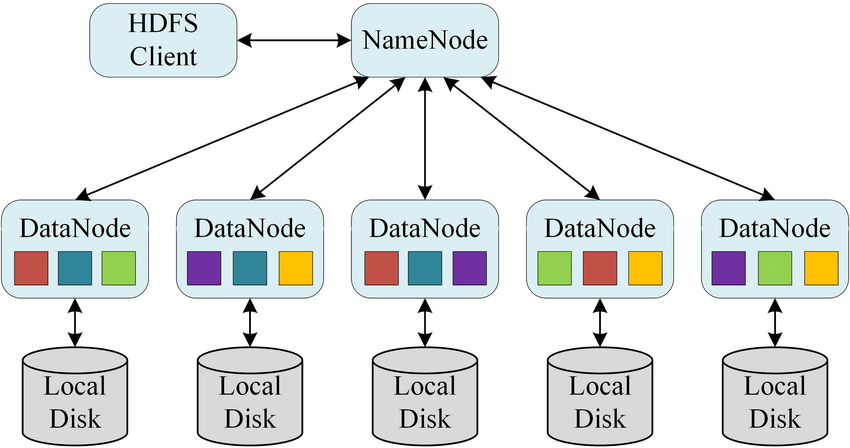
\includegraphics[width=\textwidth]{Figures/1. Content/Hadoop-Distributed-File-System-HDFS.ppm}
        \caption{Hadoop Distributed File System (HDFS) Overview Architecture}
        \label{fig: HDFSArchitecture}
    \end{subfigure}
    \hfill
\end{figure}

El Hadoop Distributed File System (HDFS) es otro sistema DFS de gran relevancia, diseñado para trabajar con el framework de MapReduce. HDFS es conocido por su capacidad de almacenar enormes conjuntos de datos, su modelo de replicación para garantizar la disponibilidad de datos, y su arquitectura que permite la distribución efectiva y la replicación de los datos en múltiples nodos.

\subsection{Principios Clave de HDFS}

El Hadoop Distributed File System (HDFS) es un sistema de archivos diseñado para almacenar grandes conjuntos de datos de manera confiable y eficiente. Su arquitectura se compone de un NameNode y múltiples DataNodes.

\subsubsection{Arquitectura:}

\begin{itemize}
    \item \textbf{NameNode:} Mantiene y gestiona el espacio de nombres del sistema de archivos. Guarda la metadata, como la estructura del árbol de archivos, permisos, y el mapeo de archivos a bloques de datos.
    \item \textbf{DataNodes:} Almacenan los datos efectivos en forma de bloques (usualmente de 128 MB). Cada bloque de datos se replica en varios DataNodes según la política de replicación.
\end{itemize}

\subsubsection{Coherencia y Replicación:}

\begin{itemize}
    \item HDFS se basa en un modelo de escritura una vez, lectura muchas veces (WORM). Esto significa que una vez que un archivo se escribe, no se puede modificar, solo leer o agregar más datos.
    \item La replicación de datos en múltiples DataNodes proporciona tolerancia a fallos y alta disponibilidad. HDFS también realiza un balanceo y redistribución de bloques para optimizar el almacenamiento y el acceso a los datos.
\end{itemize}

\subsubsection{Características útiles para el desarrollo de "Azeroth Nodes":}

\begin{itemize}
    \item Considerando la eficiencia de HDFS en el manejo de grandes datos, su integración con sistemas de procesamiento como MapReduce puede ser un punto de referencia valioso para "Azeroth Nodes".
    \item La arquitectura de HDFS con un NameNode central y múltiples DataNodes proporciona un modelo claro para la gestión y el almacenamiento distribuido, que puede ser adaptado en "Azeroth Nodes" para mejorar la escalabilidad y el rendimiento.
\section{Comparación y Contraste entre GFS y HDFS}

Aunque GFS y HDFS comparten similitudes en términos de ser sistemas de archivos distribuidos diseñados para manejar grandes conjuntos de datos, tienen diferencias significativas en términos de arquitectura y manejo de operaciones. Por ejemplo, GFS fue diseñado específicamente para las necesidades internas de Google, mientras que HDFS es un proyecto de código abierto, parte de Apache Hadoop, y es ampliamente utilizado en muchas aplicaciones de procesamiento de datos.

\section{Impacto en el Desarrollo de Aplicaciones de Big Data}

Tanto GFS como HDFS han tenido un impacto considerable en el diseño y desarrollo de aplicaciones modernas de big data. Su capacidad para manejar grandes volúmenes de datos de manera eficiente y confiable ha permitido el desarrollo de soluciones avanzadas en áreas como el análisis de datos, la minería de datos y el aprendizaje automático.

\section{Aplicación a "Azeroth Nodes"}

\begin{figure}[H]
    \centering
    \begin{subfigure}[b]{0.5\textwidth}
        \centering
        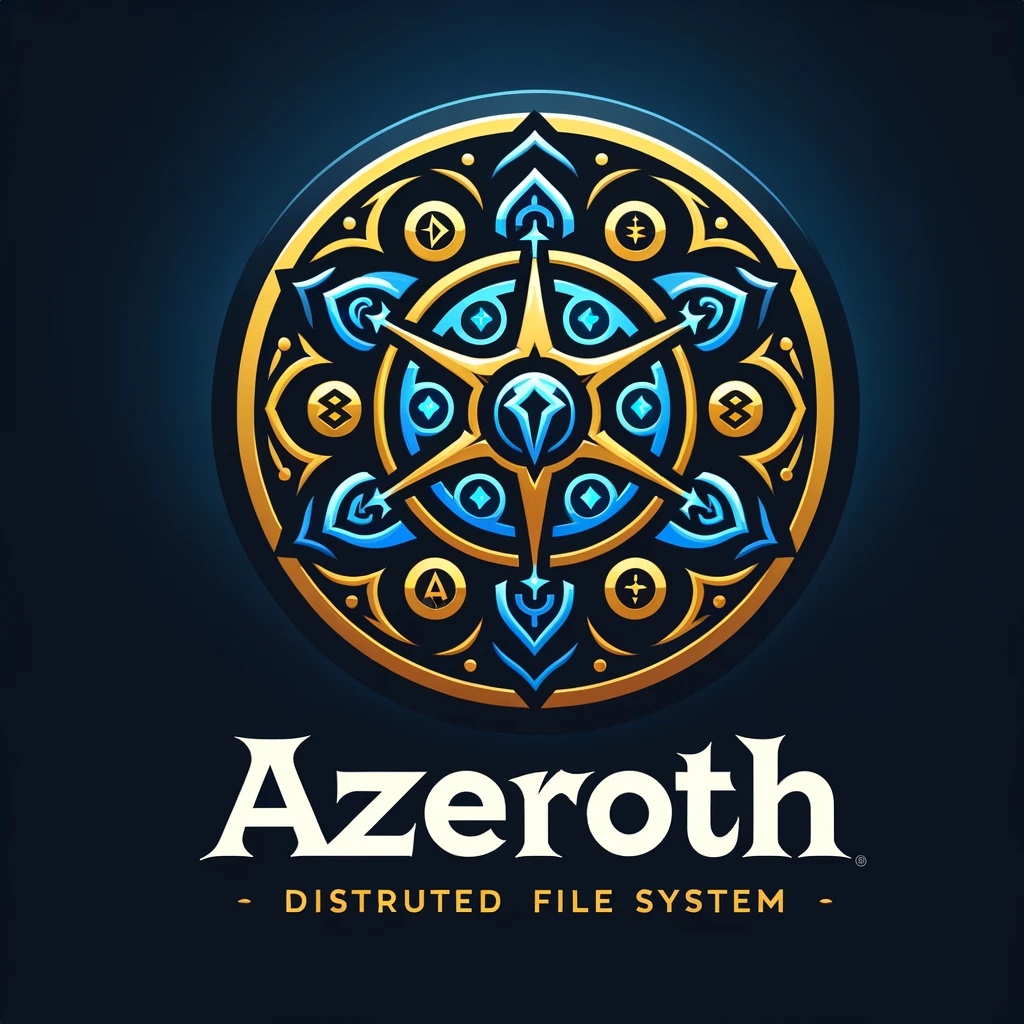
\includegraphics[width=\textwidth]{Figures/1. Content/AzerothNodes.webp}
        \caption{Azeroth Nodes Logo}
        \label{fig: Azeroth Nodes Logo}
    \end{subfigure}
    \hfill
\end{figure}

"Azeroth Nodes", un proyecto DFS inspirado en GFS y HDFS, se centra en proporcionar un sistema de archivos distribuido robusto y eficiente, utilizando el lenguaje Rust. Este sistema busca combinar las mejores prácticas y lecciones aprendidas de GFS y HDFS, implementando una arquitectura que permite una escalabilidad masiva, alta disponibilidad y seguridad en el almacenamiento y recuperación de datos. La adaptación de estos principios a "Azeroth Nodes" no solo mejora la eficiencia y confiabilidad del almacenamiento de archivos distribuidos, sino que también abre nuevas posibilidades para aplicaciones avanzadas en el ámbito de big data y la analítica de datos.\newline \hfill \break

Este marco teórico proporciona una base sólida para entender los sistemas DFS y su aplicación en "Azeroth Nodes", presentando cómo este proyecto puede ser una evolución o contribución significativa en el ámbito de almacenamiento y procesamiento de grandes volúmenes de datos.